\documentclass[12pt]{article}
\usepackage[a4paper, total={7in,10in}]{geometry}

\usepackage{polyglossia}
\usepackage{ragged2e}
\usepackage{amsmath}
\usepackage{amssymb}
\usepackage{microtype}
\usepackage{graphicx}
\usepackage{changepage}
\usepackage{hyperref}
\usepackage{cancel}
\usepackage{wrapfig}
\usepackage{needspace}
\usepackage{mathtools}
\usepackage{tikz}
\usepackage{esint}
\newcommand*\circled[1]{\tikz[baseline=(char.base)]{
    \node[shape=circle, draw, inner sep=1pt, 
        minimum height=12pt] (char) {#1};}}



\let\ORIincludegraphics\includegraphics
\renewcommand{\includegraphics}[2][]{\ORIincludegraphics[scale=0.65,#1]{#2}}
\newcommand{\verteq}{\rotatebox{90}{$\,=$}}
\newcommand{\equalto}[2]{\underset{\scriptstyle\overset{\mkern4mu\verteq}{#2}}{#1}}

\graphicspath{{./images/}}
\setmainlanguage{russian}
\setotherlanguage{english}
\newfontfamily\russianfont[Script=Cyrillic]{Times New Roman}
\newfontfamily\englishfont{Times New Roman}
\setlength{\parindent}{0em}
\setlength{\parskip}{6pt}

\def\posl#1#2{\{#1_{#2}\}}
\DeclareMathOperator*{\sh-like}{\sinh-like}
\DeclareMathOperator*{\ch-like}{\cosh-like}
\DeclareMathOperator*{\th-like}{\tanh-like}
\DeclareMathOperator*{\cth-like}{\coth-like}
\DeclareMathOperator*{\tg-like}{\tan-like}
\DeclareMathOperator*{\ctg-like}{\cot-like}
\DeclareMathOperator*{\arctg-like}{\arctan-like}
\DeclareMathOperator*{\arcctg-like}{\arctan-like}

\begin{document}
    \pagebreak
    \tableofcontents
    \pagebreak
    \section{Теория множеств}
    \justifying
    \subsection{Основные операции}
    \begin{itemize}
        \item $a \subset A$
        \item $\varnothing$
        \item $A \subset B \Leftrightarrow A \subseteq B \text{ и } \exists x (x \in B \text{ и } x\not \int A)$
        \item $A \subseteq B \Leftrightarrow \forall x (x \in A \Rightarrow x \in B)$
        \item $A \land B = \{x | x \in A \text{ и } x \in B\}$
        \item $A \lor B = \{x | x \in A \text{ или } x \in B\}$
        \item $A \ B = \{x | x\in A \text{ и } x \not \in B\}$
        \item $A \bigtriangleup B = (A \lor B)\backslash(A\land B) = (A\backslash B)\lor(B \backslash A)$
        \item $\overline{A_B} = B \backslash A = \{x \in B | x \not in A\}$
    \end{itemize}
    $A_1$x$\dots$x$A_n$=$\{(a_1,\dots,a_n) | \forall i \in n (a_i \in A_i)\}$, где ($a_1,\dots,a_n$) - упорядоченный набор, который определяется
    следующим образом:
    \begin{enumerate}
        \item $n=0 \Rightarrow \varnothing$
        \item $n=1 \Rightarrow \{a_1\}$
        \item $n=2 \Rightarrow \{\{a_1\},\{a_2\}\}(\{\{a_2\},\{a_2,a_1\}\})$
        \item $n > 2 \Rightarrow (a_1,\dots,a_{n-1},a_n)=((a_1,\dots,a_{n-1}),a_n)$
    \end{enumerate}
    \[(1,2,3)=((1,2),3)=\{\{(1,2)\},\{3\}\}=\{\{1\},\{2\},\{3\}\}=\{\{\{1\},\{1,2\}\}\},\{\{\{1\},\{1,2\}\},3\}\]
    \subsection{Бинарные отношения}
    \underline{Определение: } Множество $\rho \supseteq A_1 \text{x}\dots \text{x}A_n$ - называется n-местным отношением на ($A_1,\dots,A_n$)
    (n>0). Если $A_1 =A_2 = \dots = A_n = A$, то $\rho$ называется n-местным отношением на A. Если n=2, то $\rho$ называется бинарным отношением.
    \subsection*{Пример:}
    \[A=\{1,2,3\}\]
    \[B=\{a,b\}\]
    \[A \text{ x } B = \{(1;a),(2;a),(3;a),(1,b),(2,b),(3,b)\}\]
    \[B \text{ x } A = \{(a;1),(a;2),(a;3),(b,1),(b,2),(b,3)\}\]
    \begin{itemize}
        \item $\rho_1,\rho_2 \subseteq A \text{ x } B$
        \item $\rho_1 = \{(1;a),(1;b)\}$
        \item $\rho_2 = \{(1;a),(1;b),(2;b)\}$
        \item $\rho_3 \subseteq A^2$
        \item $\rho_3 = \{(1,1),(1,2),(3;1)\}$
        \item $\rho_4,\rho_5 \subseteq A \text{ x } B \text{ x } A$
        \item $\rho_4 = \{(1,b,2),(3,a,1)\}$
        \item $\rho_5 = \varnothing$
    \end{itemize}
    \underline{Определение: } Пусть $\rho$ = A x B
    \[\text{Dom}(\rho)\overset{\text{def}}{=}\{x \in A | \exists y \in B:(x,y) \in \rho\} \text{ - область определения}\]
    \[\text{Im}(\rho)\overset{\text{def}}{=}\{y \in B | \exists x \in A:(x,y)\in \rho\} \text{ - область значений}\]
    \[\rho^{-1}\overset{\text{def}}{=} \{(y,x)\in B \text{ x } A | (x,y)\in \rho\} \text{ - обратное к } \rho\]
    \underline{Пример:} 
    \[\text{Dom}(\rho_2)=\{1,2\}\]
    \[\text{Im}(\rho_2)=\{a,b\}\]
    \[\rho^{-1}=\{(a,1),(b,1),(b,2)\}\]
    \subsection*{Своства бинарный отнешений на A:}
    Пусть $\rho \subseteq A^2$. Тогда:
    \begin{enumerate}
        \item $\rho$ - рефлексивное $\overset{\text{def}}{\Leftrightarrow} \forall x \in A ((x,x)\in \rho)$
        \item $\rho$ - симметричное $\overset{\text{def}}{\Leftrightarrow} \forall x \in A ((x,y)\in \rho \Rightarrow (y,x) \in \rho)$
        \item $\rho$ - транзитивно $\overset{\text{def}}{\Leftrightarrow} \forall x,y,z \in A ((x,y)\in \rho \text{ и } (y,z)\in \rho
        \Rightarrow (x,z) \in \rho)$
        \item $\rho$ - антирефлексивно $\overset{\text{def}}{\Leftrightarrow} \forall x \in A ((x,x) \not \in \rho)$
        \item $\rho$ - антисиметрично $\overset{\text{def}}{\Leftrightarrow} \forall x \in A (x \not = y \text{ и } (x,y) \in \rho
        \Rightarrow (y,x)\not \in \rho)$
        \item $\rho$ - связное $\overset{\text{def}}{\Leftrightarrow}\forall x,y \in A (x \not = y \Rightarrow (x,y)\in \rho \text{ или }
        (y,x)\in \rho)$
    \end{enumerate}
    \subsection{Отношение эквивалентности}
    \underline{Определение: } Бинарное отношение $\rho \subseteq A^2$ называется отношением эквивалентности, если оно рефлексивно,
    симметрично и транзитивно.\\
    \underline{Пример:} 
    \begin{enumerate}
        \item $\overset{5}{\equiv}$ на Z\\
        $x \underset{5}{\equiv} y \Leftrightarrow x-y \vdots 5$
        \begin{enumerate}
            \item $x-x \vdots 5 \Rightarrow x \equiv x $ рефлексивно
            \item $x \underset{5}{\equiv} \Rightarrow x-y\vdots 5 \Rightarrow y-x \vdots 5 \Rightarrow y \underset{5}{\equiv} x $ симметрично
            \item $x \underset{5}{\equiv} y \Rightarrow x-y\vdots 5$
            \[y\underset{5}{\equiv}z\Rightarrow \frac{y-z\vdots 5}{x-z\vdots 5}\Rightarrow x \underset{5}{\equiv} z \] транзитивно
        \end{enumerate}
        \item  А - множество всех студентов в аудитории E702.\\
        \begin{minipage}{0.3\textwidth}
            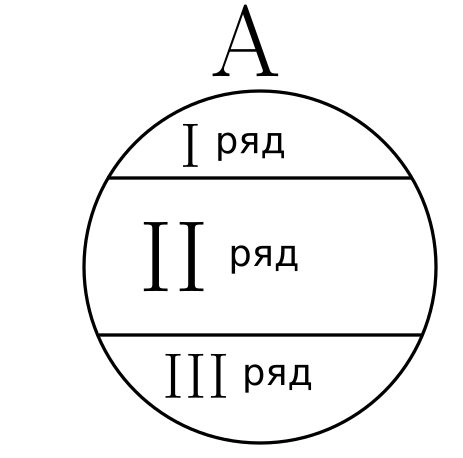
\includegraphics[scale=0.3]{1.1.png}
        \end{minipage}
        \hspace{1em}
        \begin{minipage}{0.7\textwidth}
            $<x,y> \in \rho \overset{\text{def}}{\Leftrightarrow}$ x и y сидят в одном ряду\\
            \par
        $\rho$ - рефлексивно, симметрично, транзитивно $\Rightarrow$\\$\rho$- отношение эквивалентности
        \end{minipage}
        \begin{minipage}{0.55\textwidth}
            \item А - множество $\bigtriangleup$ плоскости\\
            $<\bigtriangleup_1,\bigtriangleup_2> \in \rho \overset{\text{def}}{\Leftrightarrow}$\\
            $\rho - \text{ отношение эквивалентности }$\\
        \end{minipage}
        \begin{minipage}{0.45\textwidth}
            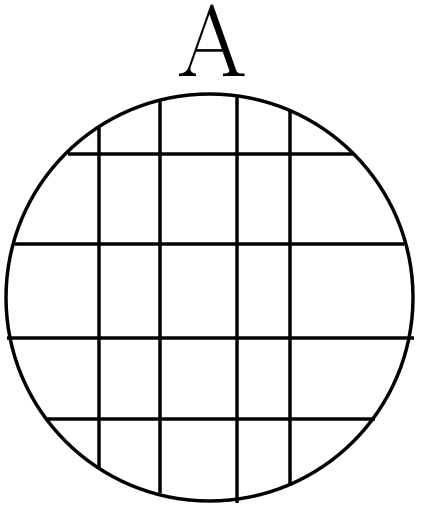
\includegraphics[scale=0.3]{1.2.png}
        \end{minipage}
        \hspace{1em}
        \vspace{1em}
        \par
    \end{enumerate}
    \underline{Определение: } Пусть $\rho$ - отношение эквивалентности на А, $a \in A$. Множество \\
    $\frac{a}{\rho}$=$\{x \in A | <a,x> \in \rho\}$ называется классов эквивалентности с представителем
    \subsubsection*{Теорема 1}\label{th:1}
    \par\noindent
    Пусть $\rho$ - эквивалентность на А, a и b $\in A$. Тогда $<a,b> \in \rho \Leftrightarrow \frac{a}{\rho}=\frac{b}{\rho}.$\\
    \par\noindent
    \underline{Доказательство:}
    \begin{adjustwidth}{1.5em}{1.5em}
        $\boxed{\Rightarrow}$ Пусть $x \in \frac{a}{\rho}.$ По определению $<a,x> \in \overset{(1)}{\rho}$. \\
        Так как $<a,b>\in \rho$ и $\rho$ - симметрично, то $<b,a> \in \overset{(2)}{\rho}$\\
        (1)(2) $\underset{\rho \text{ - транзитивно}}{\Rightarrow} <b,x> \in \rho \Rightarrow x \in \frac{b}{\rho}$.\\
        То $\frac{a}{\rho} \subseteq \frac{b}{\rho}.$ Аналогично, $\frac{b}{\rho} \subseteq \frac{a}{\rho}$. 
        Следовательно $\frac{a}{\rho}=\frac{b}{\rho}$\\
        $\boxed{\Leftarrow}$ Так как - $\rho$ рефлексивно, то $<a,a> \in \rho,$ то есть $a \in \frac{a}{\rho}$.\\
        Из $\frac{a}{\rho}=\frac{b}{\rho}$ следует, что $a \in \frac{b}{\rho}.$ Поэтому $<b,a> \in \rho$, и за счёт
        метричности $\rho$ получим, что $<a,b> \in \rho$
    \end{adjustwidth}
    \begin{center}
        \textbf{Ч.т.д.}
    \end{center}
\end{document}